\section{Methodology and Implementation}
\label{sec:method}

\subsection{Hardware Platform and Board Selection}
\label{sec:method:boards}

Three embedded targets were evaluated in order before obtaining clean
power measurements:

\paragraph{Raspberry Pi Pico (RP2040, Cortex-M0+, 125\,MHz).}
The RP2040 contains an on-chip \textbf{Switch-Mode Power Supply (SMPS)}
that steps the 3.3\,V USB supply to $\approx$1.1\,V DVDD for the processor
cores~\cite{rp2040datasheet}.
The SMPS switching frequency ($\approx$1\,MHz) injects broadband noise
directly onto the DVDD rail, masking the data-dependent AES leakage signal
which is a $\mu$A-level current modulation.
Variance analysis on 100 captured traces showed the AES computation window
occupies only 20\,\% of the acquisition and the peak-variance SNR proxy
was $\approx$$21\times$ above the noise floor---insufficient for attack
convergence.
Bypassing the SMPS (the approach used by ChipWhisperer's CW308 UFO board)
was not attempted.

\begin{figure}[H]
  \centering
  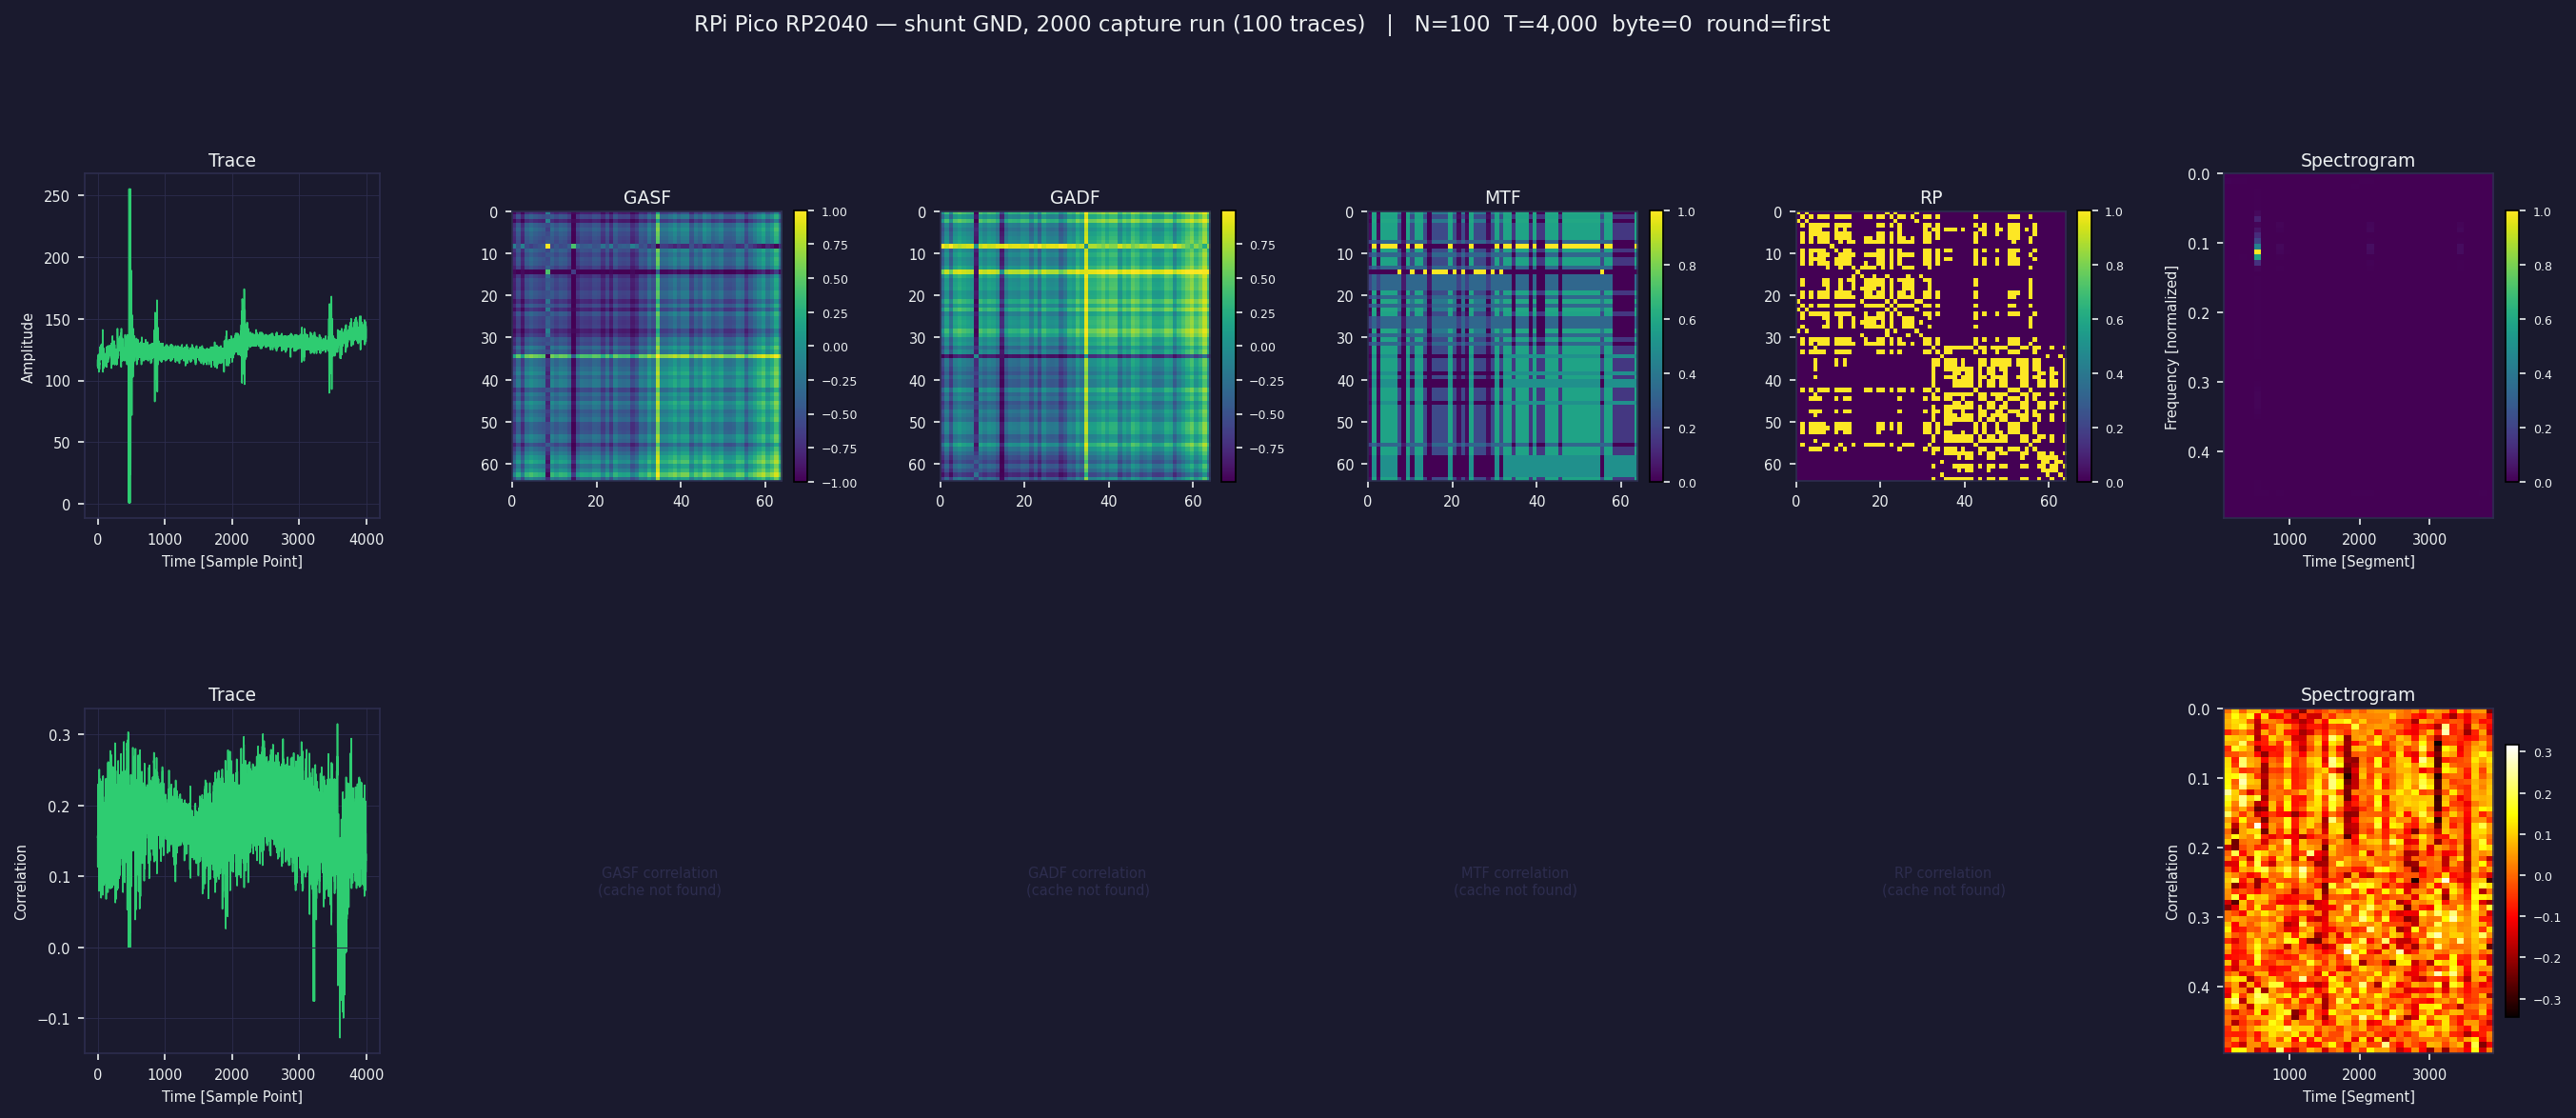
\includegraphics[width=\linewidth]{figures/pico_data_view.png}
  \caption{Data overview for RPi Pico real capture (\texttt{set\_001\_pico\_real}).
           Top row: raw trace overlay, mean trace, variance trace.
           The AES computation window is buried in SMPS switching noise
           with no visible data-dependent structure.}
  \label{fig:pico_data_view}
\end{figure}

% The trigger alignment figure (media/diagnostics/trigger_alignment.png)
% quantifies the SNR difference between Pico and Trinket.
% Copy to report/figures/trigger_alignment.png and uncomment:
%
% \begin{figure}[H]
%   \centering
%   \includegraphics[width=\linewidth]{figures/trigger_alignment.png}
%   \caption{Variance analysis: RPi Pico vs.\ Pro Tinkrer trace sets.
%            Peak-variance SNR proxy: Pico $\approx$$21\times$,
%            Trinket $\approx$$78\times$.
%            The AES window is barely distinguishable from the noise floor
%            on the Pico but clearly visible on the Trinket.}
%   \label{fig:trigger_alignment}
% \end{figure}

\paragraph{Arduino Uno R4 Minima (Renesas RA4M1, Cortex-M4, 48\,MHz).}
The RA4M1 also has internal DC-DC power regulation.
2{,}000 traces were captured (shunt on the GND rail, 4{,}807 samples each),
but neither CPA nor DPA converged.
AVR/Cortex-M targets typically require $>$5{,}000 traces for first-round
attacks; the noisy baseline from the internal regulator and the limited
trace count together prevented key recovery.

\paragraph{Adafruit Pro Tinkrer 5\,V @ 16\,MHz (ATmega328P).}
The ATmega328P runs directly from the 5\,V USB rail through a
linear Schottky diode (MBR0520), with no
SMPS~\cite{adafruit_trinket_pro,atmega328p}.
A 10\,$\Omega$ shunt in series with the VCC pin provides a clean differential
voltage proportional to processor current.
This device is the successful real-hardware capture target;
Traces in different data capture runs were collected in 2000 all 10 rounds, 200 (all 10 AES rounds) and 2000 (only first AES round) and 200 (only first AES round) (see Table~\ref{tab:boards}), a special segmented set of 10000 traces of first round were also collected at reduced sampling rate (see Table~\ref{tab:boards}).

\begin{table}[H]
\centering
\caption{Board progression summary.}
\label{tab:boards}
\begin{tabular}{@{}llll@{}}
\toprule
Board & MCU & Traces captured & Outcome \\
\midrule
RPi Pico & RP2040 (Cortex-M0+, 125\,MHz) & 100 & Failed — SMPS noise \\
Arduino Uno R4 & RA4M1 (Cortex-M4, 48\,MHz) & 2{,}000 & Failed — insufficient $N$ \\
\textbf{Pro Tinkrer 5\,V} & \textbf{ATmega328P (16\,MHz)} & 2{,}000 \& 10000 \& 2000 First-Round & \textbf{Success} \\
Reference dataset & CW-target (unknown) & 2{,}000 & \textbf{Success} \\
\bottomrule
\end{tabular}
\end{table}

The primary quantitative analysis in this report uses the
\textbf{dpa-on-aes reference dataset}
(Section~\ref{sec:method:ref}) to validate the attack implementations
against a known-good capture before applying them to oscilloscope data.

\subsection{Target Firmware}
\label{sec:method:fw}

Custom firmware follows the same pattern across all three boards: wait for
16 bytes of plaintext over serial, assert a GPIO trigger high, run
\texttt{AES\_ECB\_encrypt} via \texttt{tiny-AES-c}~\cite{tinyaes},
assert the trigger low, and return the 16-byte ciphertext.

\begin{lstlisting}[language=C, caption={Trigger and encryption loop (all targets)}]
gpio_put(TRIGGER_PIN, 1);    // Trigger HIGH before AES
AES_ECB_encrypt(&ctx, plaintext);
gpio_put(TRIGGER_PIN, 0);    // Trigger LOW after AES
\end{lstlisting}

On the \textbf{Pro Tinkrer } the trigger is GPIO\,8; the firmware is
compiled with the AVR-GCC toolchain and flashed via the Arduino bootloader.

The hardcoded 128-bit profiling key is:
\texttt{2B 7E 15 16 28 AE D2 A6 AB F7 15 88 09 CF 4F 3C}.

\subsection{Data Acquisition}
\label{sec:method:acq}

The host-side script (\texttt{capture/capture.py}) coordinates the
oscilloscope and target over USB-UART.
Oscilloscope control uses the \texttt{pyvisa} library with a PyVISA-py
backend (USBTMC, Keysight VISA address
\texttt{USB0::0x2A8D::0x17B6::MY65060127::INSTR}).

\textbf{Pro Tinkrer hardware configuration:}
\begin{itemize}
  \item \textbf{Shunt:} 10\,$\Omega$ in series with the Trinket VCC pin
        (5\,V rail); oscilloscope CH1 reads differential voltage across
        the shunt.
  \item \textbf{Trigger:} GPIO\,8 rising edge on scope CH2 / EXT TRIG BNC.
  \item \textbf{Sample rate:} $\geq$\,250\,MS/s; \textbf{30{,}000 points}
        per acquisition (binary BYTE format).
  \item \textbf{Serial:} USB-UART FTDI adapter, 115200 baud,
        \texttt{/dev/tty.usbserial-XXXX}.
\end{itemize}

Acquisition loop:
\begin{enumerate}
  \item Configure scope: \texttt{:WAVeform:FORMat BYTE},
        \texttt{:WAVeform:POINts 30000}.
  \item For each trace: arm scope (\texttt{:SINGle}), generate random
        16-byte plaintext (\texttt{os.urandom(16)}), send over serial.
  \item GPIO\,8 rising edge triggers the scope.
  \item After ciphertext return, \texttt{*OPC?} synchronises; download
        waveform with \texttt{:WAVeform:DATA?}.
  \item Failed acquisitions (serial drop, scope timeout) are retried.
\end{enumerate}

Captured data is saved as \texttt{traces.npy} $(N \times T)$~float32,
\texttt{plaintexts.npy} $(N \times 16)$~uint8,
\texttt{ciphertexts.npy} $(N \times 16)$~uint8.

\subsection{Reference Dataset}
\label{sec:method:ref}

Real Pro Tinkrer captures exist (\texttt{set\_003} and \texttt{set\_013};
see Section~\ref{sec:method:boards}) but top up to 50{,}000 traces is still
planned for the deep learning evaluation.
As a complementary validation baseline the publicly available
\textbf{dpa-on-aes} reference dataset~\cite{oflynn2015chipwhisperer} is
also used; its pre-aligned ChipWhisperer capture provides a known-good
ground truth for the attack implementations:

\begin{itemize}
  \item $N = 2{,}000$ AES-128 ECB encryptions.
  \item $T = 29{,}000$ samples per trace (float32, range $\approx[-1278, +1373]$).
  \item Leakage type: \textbf{last-round} --- SubBytes$_{10}$ on ciphertext
        via $S^{-1}(c_b \oplus k_{10,b})$.
  \item Known key: \texttt{2B 7E 15 16 28 AE D2 A6 AB F7 15 88 09 CF 4F 3C}.
\end{itemize}

The dataset was originally distributed as per-trace text files;
we converted it to the project's \texttt{.npy} format
(\texttt{data/set\_002\_reference/}).

\subsection{Classical Attack Algorithms}
\label{sec:method:attack}

Both attacks target the \textbf{last round} of AES using ciphertexts.
After recovering the 16-byte round-10 key, the original key is recovered
via backward key schedule.

\subsubsection{Correlation Power Analysis (CPA)}

CPA uses the Pearson correlation coefficient between the hypothetical power
consumption vector $\mathbf{h}_j$ and each column $\mathbf{t}_i$ of the
trace matrix.
Following the proposal notation~\cite{brier2004cpa}:

\begin{equation}
  r_{i,j} = \frac{\displaystyle\sum_{d=1}^{D}
    \bigl(t_{d,i} - \bar{t}_i\bigr)\bigl(h_{d,j} - \bar{h}_j\bigr)}
  {\sqrt{\displaystyle\sum_{d=1}^{D}\bigl(t_{d,i}-\bar{t}_i\bigr)^2
         \cdot \sum_{d=1}^{D}\bigl(h_{d,j}-\bar{h}_j\bigr)^2}}
  \label{eq:cpa}
\end{equation}

where:
\begin{align*}
  d \in [1,D]   &\quad \text{trace index (}D\text{ total traces)}, \\
  i             &\quad \text{time-sample index}, \\
  j \in [0,255] &\quad \text{key-byte hypothesis}, \\
  t_{d,i}       &\quad \text{measured power at sample }i\text{ in trace }d, \\
  h_{d,j}       &= \mathrm{HW}\!\bigl(S^{-1}(c_{d,b} \oplus j) \oplus c\bigr),
                    \quad c \in \{0,\ldots,255\}\text{ (leakage constant)}.
\end{align*}

The predicted key byte for position $b$ is
$\hat{k}_b = \arg\max_j \max_i |r_{i,j}|$.
The leakage constant $c$ is swept from 0 to 255; the first value that
recovers a key verifying under the backward key schedule is used.
Implemented in \texttt{attacks/classical/cpa.py}.

\subsubsection{Differential Power Analysis (DPA)}

DPA partitions traces into two sets based on a predicted bit of the
intermediate value and measures the differential mean~\cite{kocher1999dpa}:

\begin{equation}
  \Delta_j = \max_i \left|
    \underbrace{\frac{1}{|S_1|}\sum_{d \in S_1} t_{d,i}}_{\text{bit}=1}
    -
    \underbrace{\frac{1}{|S_0|}\sum_{d \in S_0} t_{d,i}}_{\text{bit}=0}
  \right|
  \label{eq:dpa}
\end{equation}

where $S_1 = \{d : \mathrm{bit}_\ell(v_{d,j}) = 1\}$,
$S_0 = \{d : \mathrm{bit}_\ell(v_{d,j}) = 0\}$, and
$v_{d,j} = S^{-1}(c_{d,b} \oplus j)$.
The bit position $\ell$ is swept from 0 to 7; the first $\ell$ producing a
verifiable key is used.
Implemented with a fully vectorised matrix multiply
($T \!\times\! D$)$\cdot$($D\!\times\!256$) in \texttt{attacks/classical/dpa.py}.

\subsection{Evaluation Metrics}
\label{sec:method:metrics}

\paragraph{Guessing Entropy (GE).}
The primary metric, following~\cite{benadjila2020ascad}:
\begin{equation}
  \mathrm{GE}(N) = \mathbb{E}\bigl[\mathrm{rank}(\hat{k}_b^{(N)})\bigr]
  \label{eq:ge}
\end{equation}
where $\mathrm{rank}(\hat{k}_b^{(N)})$ is the position of the correct key
byte among 256 hypotheses sorted by descending score, after $N$ traces.
$\mathrm{GE}$ is estimated over multiple random subsets of size $N$.
$\mathrm{GE} = 1$ means full convergence.
Script: \texttt{attacks/classical/guessing\_entropy.py}.

\paragraph{Trace Complexity ($N_\text{traces}$).}
Minimum $N$ at which $\mathrm{GE}(N) \leq 1.5$.

\subsection{Deep Learning Extension: Image Encoding and CNN}
\label{sec:method:dl}

We reproduce the image-encoding SCA pipeline of Hettwer et al.\
(IEEE HOST 2020)~\cite{hettwer2020encoding}, implemented in
\texttt{attacks/deep\_learning/}.

\subsubsection{Motivation}

Standard 1D CNNs on raw power traces are sensitive to trigger jitter
that shifts the leakage point in time.
Hettwer et al.\ propose converting each 1D trace into a \textbf{2D image}
before classification: pairwise temporal correlations become spatial
textures that 2D convolutional filters detect robustly.
Small clock jitter causes a spatial translation in the image, which
Conv2D with pooling handles through translation invariance.

\subsubsection{Image Encoding Methods}

Each trace is first normalised to $x_k \in [-1,1]$ and downsampled to
$S$ samples (default $S=64$).
Let $\varphi_k = \arccos(x_k)$.
Four encodings are computed (implemented in
\texttt{attacks/deep\_learning/image\_encode.py}) and stacked as channels
of an $(S \times S \times 4)$ tensor:

\begin{description}
  \item[GASF (Gramian Angular Summation Field).]
    $\mathrm{GASF}[i,j] = \cos(\varphi_i + \varphi_j)$.
    Symmetric; diagonal $= \cos(2\varphi_k)$.
    Captures overall pairwise temporal correlation.

  \item[GADF (Gramian Angular Difference Field).]
    $\mathrm{GADF}[i,j] = \sin(\varphi_i - \varphi_j)$.
    Anti-symmetric; zero diagonal.
    Captures directionality of phase transitions.
    \textbf{GASF + GADF is the best-performing combination in the paper.}

  \item[RP (Recurrence Plot).]
    $\mathrm{RP}[i,j] = \mathbf{1}[|x_i - x_j| < \varepsilon]$,
    $\varepsilon = 0.1$.
    Encodes self-similarity; AES round periodicity produces regular
    diagonal stripe patterns useful for detecting round structure.

  \item[MTF (Markov Transition Field).]
    Quantises trace into $n=8$ bins, builds a state-transition probability
    matrix $Q$, assigns $\mathrm{MTF}[i,j] = Q[\mathrm{bin}(x_i),
    \mathrm{bin}(x_j)]$.
    Captures temporal state dynamics.
\end{description}

\subsubsection{CNN Architecture (Table~II of Hettwer et al.\ 2020)}

The classifier takes an $(S \times S \times C)$ image and outputs a
256-class softmax over S-Box intermediate values
(Table~\ref{tab:hettwer_cnn}).
Implemented exactly in \texttt{build\_hettwer\_model()} within
\texttt{hettwer\_sca.py}.

\begin{table}[H]
\centering
\caption{CNN architecture from Hettwer et al.\ 2020, Table~II.
         $C=1$ for single-channel, $C=2$ for GASF+GADF.
         Total trainable parameters ($C=2$): $\approx$1.09\,M.}
\label{tab:hettwer_cnn}
\begin{tabular}{@{}p{7.5cm}ll@{}}
\toprule
Layer & Output shape & Parameters \\
\midrule
Input & $(64, 64, C)$ & --- \\
Conv2D(8, $5{\times}5$, L2=0.01) + BatchNorm + ReLU & $(64,64,8)$ &
  $200C{+}8{+}32$ \\
MaxPool($2{\times}2$, stride 2) + Dropout(0.5) & $(32,32,8)$ & --- \\
Conv2D(16, $3{\times}3$, L2=0.01) + BatchNorm + ReLU & $(32,32,16)$ &
  $1{,}168{+}64$ \\
MaxPool($2{\times}2$, stride 2) + Dropout(0.5) & $(16,16,16)$ & --- \\
Flatten & $(4096,)$ & --- \\
Dense(250, ReLU) + BatchNorm + Dropout(0.3) & $(250,)$ &
  $1{,}024{,}250{+}1{,}000$ \\
Dense(256, Softmax) & $(256,)$ & $64{,}256$ \\
\bottomrule
\end{tabular}
\end{table}

Training: Adam ($\eta = 0.0002$), categorical cross-entropy,
early stopping (patience = 20 on \texttt{val\_loss}),
best-weights checkpoint saved to \texttt{.keras}.

\subsubsection{Key Guessing Entropy (KGE)}

The trained model outputs
$\hat{P}(S[p_{d,b} \oplus k] \mid \text{trace}_d) \in \mathbb{R}^{256}$
for each attack trace $d$.
Log-likelihoods are accumulated per key hypothesis $k$:

\begin{equation}
  \mathrm{score}[k] \mathrel{+}=
    \log \hat{P}\!\bigl(S[p_{d,b} \oplus k] \;\big|\; \text{trace}_d\bigr)
  \label{eq:kge_score}
\end{equation}

Key Guessing Entropy (KGE) is defined identically to GE
(Equation~\ref{eq:ge}): the mean rank of the correct key byte after
accumulating $N$ attack traces, averaged over $n_\text{trials}=10$ random
permutations.
The KGE curve produced by \texttt{ge\_attack()} in
\texttt{hettwer\_sca.py} corresponds directly to Figure~4 of
Hettwer et al.~\cite{hettwer2020encoding}.

Usage:
\begin{lstlisting}[language=bash, caption={Train and evaluate Hettwer CNN}]
python attacks/deep_learning/hettwer_sca.py \
    --data data/set_002_reference \
    --round last --channels gasf+gadf --byte 0
\end{lstlisting}
